\documentclass{article}
\usepackage[margin=1in]{geometry}

% Recommended, but optional, packages for figures and better typesetting:
\usepackage{microtype}
\usepackage{graphicx}
\usepackage{authblk}
\usepackage{subcaption}
\usepackage{natbib}
\usepackage{booktabs} % for professional tables
\usepackage{etoc}
\usepackage{titletoc}
\usepackage{parskip}
\setlength{\parindent}{0pt}
% hyperref makes hyperlinks in the resulting PDF.
% If your build breaks (sometimes temporarily if a hyperlink spans a page)
% please comment out the following usepackage line and replace
% \usepackage{icml2026} with \usepackage[nohyperref]{icml2026} above.
\usepackage{hyperref}
\hypersetup{colorlinks=true, linkcolor=blue, citecolor=blue, urlcolor=blue}
% Use the following line for the initial blind version submitted for review:

% For preprint, use
% \usepackage[preprint]{icml2026}

% If accepted, instead use the following line for the camera-ready submission:
% \usepackage[accepted]{icml2026}

\usepackage{amsmath}
\usepackage{amssymb}
\usepackage{mathtools}
\usepackage{amsthm}


% if you use cleveref..
\usepackage[capitalize,noabbrev]{cleveref}



% Todonotes is useful during development; simply uncomment the next line
%    and comment out the line below the next line to turn off comments
%\usepackage[disable,textsize=tiny]{todonotes}
\usepackage[textsize=tiny]{todonotes}
\usepackage{tcolorbox}
%\usepackage{hyperref}
\usepackage{url}
\usepackage{amsthm}
\usepackage{subcaption}
\usepackage{cancel}
% Graph
\def\gA{{\mathcal{A}}}
\def\gB{{\mathcal{B}}}
\def\gC{{\mathcal{C}}}
\def\gD{{\mathcal{D}}}
\def\gE{{\mathcal{E}}}
\def\gF{{\mathcal{F}}}
\def\gG{{\mathcal{G}}}
\def\gH{{\mathcal{H}}}
\def\gI{{\mathcal{I}}}
\def\gJ{{\mathcal{J}}}
\def\gK{{\mathcal{K}}}
\def\gL{{\mathcal{L}}}
\def\gM{{\mathcal{M}}}
\def\gN{{\mathcal{N}}}
\def\gO{{\mathcal{O}}}
\def\gP{{\mathcal{P}}}
\def\gQ{{\mathcal{Q}}}
\def\gR{{\mathcal{R}}}
\def\gS{{\mathcal{S}}}
\def\gT{{\mathcal{T}}}
\def\gU{{\mathcal{U}}}
\def\gV{{\mathcal{V}}}
\def\gW{{\mathcal{W}}}
\def\gX{{\mathcal{X}}}
\def\gY{{\mathcal{Y}}}
\def\gZ{{\mathcal{Z}}}
%\def\piref{\pi_{\mathrm{ref}}}
%\def\piout{\pi_{\mathrm{out}}}
\def\sP{{\mathbb{P}}}
\def\sD{{\mathbb{D}}}

%\usepackage[unicode,psdextra]{hyperref}
\usepackage{wrapfig}
% Parentheses
\newcommand{\abs}[1]{\left |{#1}\right |}
\newcommand{\bc}[1]{\left\{{#1}\right\}}
\newcommand{\br}[1]{\left({#1}\right)}
\newcommand{\bs}[1]{\left[{#1}\right]}
\newcommand{\ceil}[1]{\left\lceil #1 \right\rceil}
\newcommand{\floor}[1]{\left\lfloor #1 \right\rfloor}
\newcommand{\bsd}[1]{\left\llbracket{#1}\right\rrbracket}
\newcommand{\ip}[2]{\left\langle{#1},{#2}\right\rangle}
\newcommand{\inner}[1]{\langle#1\rangle}
% Statistics notation
% Probabilities
\renewcommand{\P}[1]{\mathbb{P}\bs{{#1}}}
\newcommand{\Pp}[2]{\underset{#1}{\mathbb{P}}\bs{{#2}}}
\newcommand{\Ppp}[3]{\mathbb{P}_{#1}^{#2}\bs{{#3}}}
% Expectations
\newcommand{\Ee}[2]{\underset{#1}{\mathbb{E}}\bs{{#2}}}
\newcommand{\Eee}[2]{\mathbb{E}_{#1}\bs{{#2}}}
\newcommand{\sspace}{\mcf{X}}     % state space
\newcommand{\aspace}{\mcf{A}}     % action space
\newcommand{\wspace}{\mcf{W}}     % cost weights space
\newcommand{\histspace}{\mcf{H}}
\usepackage{dsfont}% history space
% argmin and argmax


\usepackage{algorithm}
\usepackage{algorithmic}
\usepackage{multirow}
\newcounter{protocol}
\makeatletter
\newenvironment{protocol}[1][htb]{%
  \let\c@algorithm\c@protocol
  \renewcommand{\ALG@name}{Protocol}% Update algorithm name
  \begin{algorithm}[#1]%
  }{\end{algorithm}
}
\usepackage{amssymb}
\usepackage{amsfonts}
\usepackage{graphics}
\usepackage{graphicx}
\usepackage{setspace}

%\usepackage{subcaption}
%\usepackage{selectp}
%\outputonly{1-18}
% \newtheorem{theorem}
%{\protect\theoremname}
%\newtheorem*{openquestion}{Open Question}
%   \newtheorem{defn}{\protect\definitionname}
%   \newtheorem{proposition}{\protect\propositionname}
%   \newtheorem{example}{\protect\examplename}
%   \newtheorem{remark}{Remark}
%   \newtheorem{conditions}{\protect\conditionsname}
    
%     \newenvironment{proofof}[1]{\begin{proof}[{#1}]}{\end{proof}}
    
% \providecommand{\definitionname}{Definition}
% \providecommand{\examplename}{Example}

% \providecommand{\propositionname}{Proposition}
% \providecommand{\conditionsname}{Conditions}
% \providecommand{\theoremname}{Theorem}
% \providecommand{\assumptionname}{Assumption}

\def \M{\mathcal{M}}
\def \S{\mathcal{S}}

\newcommand{\sigmoid}{\sigma}
% to compile a preprint version, e.g., for submission to arXiv, add add the
% [preprint] option:
%     \usepackage[preprint]{neurips_2022}


% to compile a camera-ready version, add the [final] option, e.g.:
%     \usepackage[final]{neurips_2022}


% to avoid loading the natbib package, add option nonatbib:
%    \usepackage[nonatbib]{neurips_2022}

%commands from AK
%====================================================================================================================================================================================
%new
%state space S 
\newcommand{\qv}{\mbf{q}}
\newcommand{\dv}{\mbf{d}}
\newcommand{\dve}{\mbf{d}^E}
\newcommand{\trans}{T}
\newcommand{\qval}{\mbf{Q}}
\newcommand{\FEV}[1]{\mbs{\rho}_{\phim}(#1)}
\newcommand{\EFEV}[1]{\mbs{\rho}_{\phim}(\widehat{#1})}
%==============================================================================
%old
\newcommand{\mcf}{\mathcal}
\newcommand{\mbf}{\mathbf}
\newcommand{\mbb}{\mathbb}

\newcommand{\innerprod}[2]{\left\langle{#1},{#2}\right\rangle}

\newcommand{\apprentice}{\pi_{\textup{A}}}
\newcommand{\mbs}{\boldsymbol}
\newcommand{\cost}{r}
\newcommand{\true}{r}
\newcommand{\weight}{w}
\newcommand{\X}{\mathcal{X}}
\newcommand{\A}{\mathcal{A}}
\newcommand{\phim}{\Phi}
\newcommand{\initial}{\nu_0}

\newcommand{\wtrue}{\weight_{\textup{true}}}
 %========================================================
\newcommand{\norm}[1]{\left\| {#1} \right\|}

\usepackage[utf8]{inputenc} % allow utf-8 input
\usepackage[T1]{fontenc}    % use 8-bit T1 fonts      
\usepackage{url}            % simple URL typesetting
\usepackage{booktabs}       % professional-quality tables
\usepackage{array}                                  
\newcommand{\PreserveBackslash}[1]{\let\temp=\\#1\let\\=\temp}
%\newcolumntype{C}[1]{>{\PreserveBackslash\centering}m{#1}}
\newcolumntype{M}[1]{>{\centering\arraybackslash}m{#1}} 

\newcolumntype{C}[1]{>{\centering\arraybackslash}m{#1}}
\newcolumntype{R}[1]{>{\PreserveBackslash\raggedleft}p{#1}}
\newcolumntype{L}[1]{>{\PreserveBackslash\raggedright}p{#1}}
\usepackage{amsfonts}       % blackboard math symbols
\usepackage{nicefrac}       % compact symbols for 1/2, etc.
\usepackage{microtype}      % microtypography
\usepackage[table]{xcolor}         % colors

\usepackage{mathtools}% http://ctan.org/pkg/mathtools

\usepackage{amsthm}
\allowdisplaybreaks[4]
\usepackage{thm-restate}
%\usepackage{thmtools}
\usepackage{tcolorbox}
\usepackage{hyperref}
\hypersetup{colorlinks=true, linkcolor=blue, citecolor=blue, urlcolor=blue}
\usepackage[capitalize,noabbrev]{cleveref}
\usepackage{url}
\usepackage{subcaption}
\usepackage{cancel}

\theoremstyle{plain}
\newtheorem{theorem}{Theorem}[section]
\newtheorem{proposition}[theorem]{Proposition}
\newtheorem{lemma}[theorem]{Lemma}
\newtheorem{Lem}[theorem]{Lemma}
\newtheorem{corollary}[theorem]{Corollary}
\theoremstyle{definition}
\newtheorem{definition}[theorem]{Definition}
\newtheorem{assumption}[theorem]{Assumption}
\theoremstyle{remark}
\newtheorem{remark}[theorem]{Remark}
\crefname{assumption}{Assumption}{Assumptions}
\Crefname{assumption}{Assumption}{Assumptions}

\newtheorem{example}[theorem]{Example}
\usepackage[textsize=tiny]{todonotes}

% Graph
\def\gA{{\mathcal{A}}}
\def\gB{{\mathcal{B}}}
\def\gC{{\mathcal{C}}}
\def\gD{{\mathcal{D}}}
\def\gE{{\mathcal{E}}}
\def\gF{{\mathcal{F}}}
\def\gG{{\mathcal{G}}}
\def\gH{{\mathcal{H}}}
\def\gI{{\mathcal{I}}}
\def\gJ{{\mathcal{J}}}
\def\gK{{\mathcal{K}}}
\def\gL{{\mathcal{L}}}
\def\gM{{\mathcal{M}}}
\def\gN{{\mathcal{N}}}
\def\gO{{\mathcal{O}}}
\def\gP{{\mathcal{P}}}
\def\gQ{{\mathcal{Q}}}
\def\gR{{\mathcal{R}}}
\def\gS{{\mathcal{S}}}
\def\gT{{\mathcal{T}}}
\def\gU{{\mathcal{U}}}
\def\gV{{\mathcal{V}}}
\def\gW{{\mathcal{W}}}
\def\gX{{\mathcal{X}}}
\def\gY{{\mathcal{Y}}}
\def\gZ{{\mathcal{Z}}}
\def\piref{\pi_{\mathrm{ref}}}
\def\piout{\pi_{\mathrm{out}}}
\def\piouth{\pi_{\mathrm{out},h}}
\def\sP{{\mathbb{P}}}
\def\sD{{\mathbb{D}}}

% Till
\definecolor{mgh}{rgb}{0.1,0.5,0.1}%{0.1,0.1,0.8}
\newcommand{\mgh}[1]{{\color{mgh}{[MGH: #1]}}}
\newcommand{\mghtd}[2][inline]{\todo[color=mgh!40,#1]{MGH: #2}}
\newcommand{\mghtdd}[1]{\todo[color=mgh!40]{MGH: #1}}
\newcommand{\pidata}{\pi_{\mathrm{data}}}
% Luca
\definecolor{lu}{rgb}{0.8,0.1,0.1}
\newcommand{\lu}[1]{{\color{lu}{#1}}}
\newcommand{\lutd}[1]{\todo[color=lu!40,inline]{Lu: #1}}
\newcommand{\lutdd}[1]{\todo[color=lu!40]{Lu: #1}}

% Giorgia
\definecolor{gr}{rgb}{0.4,0.7,0.2}
\newcommand{\gr}[1]{{\color{gr}{#1}}}
\newcommand{\grtd}[2][inline]{\todo[color=gr!40,#1]{GR: #2}}
\newcommand{\grtdd}[1]{\todo[color=wa!40]{GR: #1}}

% Matthieu
\definecolor{st}{rgb}{0.1,0.5,0.1}
\newcommand{\st}[1]{{\color{st}{#1}}}
\newcommand{\sttd}[2][inline]{\todo[color=sw!40,#1]{SW: #2}}
\newcommand{\sttdd}[1]{\todo[color=sw!40]{SW: #1}}


\definecolor{greenp}{rgb}{0.0, 0.51, 0.5}

\newcommand{\argmin}{\mathop{\rm argmin}}
\newcommand{\argmax}{\mathop{\rm argmax}}

\newcommand{\expert}{\operatorname{E}}
\newcommand{\expertp}{{\pi_E}}
\newcommand{\experti}{\pi_E^i}
\newcommand{\piE}{\pi^{\expert}}
\newcommand{\muE}{\mu^{\expert}}
\newcommand{\nuE}{\nu^{\expert}}

\newcommand{\reals}{\mathbb{R}}
\newcommand{\RMAX}{R_{\max}}
\newcommand{\ptie}{\mathfrak{p}_{\mathrm{tie}}}
\newcommand{\pess}{\mathrm{pess}}
\newcommand{\RS}{\mathrm{RS}}
\usepackage{makecell}

 % MAIL quantities
 \newcommand{\cphimax}{C_{\phi, \max}}
 
 \newcommand{\fn}{\mathcal{F}_{n-1}}


% caligraphic letters
\newcommand{\cA}{\mathcal{A}}
\newcommand{\cB}{\mathcal{B}}
\newcommand{\cC}{\mathcal{C}}
\newcommand{\cD}{\mathcal{D}}
\newcommand{\cE}{\mathcal{E}}
\newcommand{\cF}{\mathcal{F}}
\newcommand{\cG}{\mathcal{G}}
\newcommand{\cH}{\mathcal{H}}
\newcommand{\cI}{\mathcal{I}}
\newcommand{\cJ}{\mathcal{J}}
\newcommand{\cK}{\mathcal{K}}
\newcommand{\cL}{\mathcal{L}}
\newcommand{\cM}{\mathcal{M}}
\newcommand{\cN}{\mathcal{N}}
\newcommand{\cO}{\mathcal{O}}
\newcommand{\cP}{\mathcal{P}}
\newcommand{\cQ}{{\mathcal{F}_Q}}
\newcommand{\cR}{\mathcal{R}}
\newcommand{\cX}{\mathcal{X}}
\newcommand{\cT}{\mathcal{T}}
\newcommand{\cU}{\mathcal{U}}
\newcommand{\cV}{\mathcal{V}}
\newcommand{\cY}{\mathcal{Y}}
\newcommand{\cZ}{\mathcal{Z}}

% blackboard bold letters
\newcommand{\bbC}{\mathbb{C}}
\newcommand{\bbE}{\mathbb{E}}
\newcommand{\bbF}{\mathbb{F}}
\newcommand{\bbI}{\mathbb{I}}
\newcommand{\bbN}{\mathbb{N}}
\newcommand{\bbP}{\mathbb{P}}
\newcommand{\bbQ}{\mathbb{Q}}
\newcommand{\bbR}{\mathbb{R}}
\newcommand{\bbRnnK}{\mathbb{R}_{\geq 0}^K}
\newcommand{\bbRpK}{\mathbb{R}_{>0}^K}
\newcommand{\bbV}{\mathbb{V}}
\newcommand{\bbZ}{\mathbb{Z}}

\newcommand{\Xeinh}{X_{\scriptscriptstyle\textup{E},h}^{n,i}}
\newcommand{\Aeinh}{A_{\scriptscriptstyle\textup{E},h}^{n,i}}
\newcommand{\tauE}{\tau_{\scriptscriptstyle\textup{E}}}

\usepackage{pifont}
\newcommand{\greentick}{\textcolor{black!30!green}{\ding{51}}}
\newcommand{\redcross}{\textcolor{red}{\ding{55}}}
\newcommand{\blackcross}{\ding{55}}
\def\sP{{\mathbb{P}}}
\def\sD{{\mathbb{D}}}

\newcommand{\lp}{\left(}
\newcommand{\rp}{\right)}
\newcommand{\lb}{\left\{}
\newcommand{\rb}{\right\}}
\newcommand{\ls}{\left[}
\newcommand{\rs}{\right]}
\newcommand{\labs}{\left|}
\newcommand{\rabs}{\right|}
\newcommand{\lnorm}{\left\|}
\newcommand{\rnorm}{\right\|}
\newcommand{\expect}{\mathbb{E}}
\def\TV{\mathrm{TV}}


\DeclarePairedDelimiter{\spr}{(}{)}
\DeclarePairedDelimiter{\sbr}{[}{]}
\DeclarePairedDelimiter{\sdbr}{[\![}{]\!]}
\DeclarePairedDelimiter{\scbr}{\{}{\}}
\newcommand{\abss}[1]{|#1|}                          %absolute value
\newcommand{\normm}[1]{\lVert#1\rVert}               %norm
\newcommand{\normbig}[1]{\big\lVert#1\big\rVert}
\newcommand{\half}{\tfrac{1}{2}}

%\newcommand{\scbr}[1]{\left\{ #1 \right\}}
\newcommand{\inp}[1]{\left\langle #1 \right\rangle}

% basic algebra symbols
\newcommand{\sumiK}{\sum_{i=1}^K}
\newcommand{\sumjK}{\sum_{j=1}^K}
\newcommand{\sumkK}{\sum_{k=1}^K}
\newcommand{\sumtT}{\sum_{t=1}^T}
\newcommand{\sumst}{\sum_{s=1}^t}
\newcommand{\sumtinfty}{\sum_{t=0}^\infty}
\newcommand{\sumsinfty}{\sum_{s=0}^\infty}

\usepackage{tikz}
\usetikzlibrary{automata,arrows, positioning,shapes.geometric, arrows.meta, shadows}

%%%%% GERGO %%%%
\newcommand{\grg}[1]{\textcolor{red}{[\textbf{Grg:} #1]}}
\newcommand{\dd}{\mathrm{d}}

\newcommand{\raviUCB}{RAVI-UCB \xspace}
\newcommand{\RMAXalg}{RMAX \xspace}
\newcommand{\algname}{RMAX-RAVI-UCB \xspace}

\newcommand{\D}[2]{D\pa{#1\middle\|#2}}
\newcommand{\DDKL}[2]{D_{\mathrm{KL}}\pa{#1\middle\|#2}}
%\newcommand{\CB}{\mbox{CB}}
\newcommand{\CC}{\mathcal{C}}
\newcommand{\TT}{\mathcal{T}}
\newcommand{\GG}{\mathcal{G}}
\newcommand{\tGG}{\wt{\GG}}
\newcommand{\ttheta}{\wt{\theta}}
\newcommand{\btheta}{\overline{\theta}}
\newcommand{\tlambda}{\wt{\lambda}}
\newcommand{\blambda}{\overline{\lambda}}
\newcommand{\bmu}{\overline{\mu}}
\newcommand{\tQ}{\wt{Q}}
\newcommand{\tV}{\wt{V}}
\newcommand{\tpi}{\wt{\pi}}
\newcommand{\td}{\wt{d}}
\newcommand{\tr}{r^+}
\newcommand{\thr}{{\hr}^+}
\newcommand{\trho}{\wt{\rho}}
\newcommand{\trunc}[2]{\left[#1\right]_{#2}}


\newcommand{\Plin}{\mathcal{P}_{\Phi}}


\newcommand{\Hil}{\mathcal{H}}
\newcommand{\F}{\mathcal{F}}
\newcommand{\N}{\mathcal{N}}
\newcommand{\LL}{\mathcal{L}}
\newcommand{\real}{\mathbb{R}}
\newcommand{\Dw}{\mathcal{D}}
%\newcommand{\Sw}{\mathcal{S}}
\newcommand{\Rw}{\mathcal{R}}
\newcommand{\HH}{\mathcal{H}}
\newcommand{\DD}{\mathcal{D}}
\newcommand{\OO}{\mathcal{O}}
\newcommand{\tOO}{\wt{\OO}}
\newcommand{\trace}[1]{\mbox{tr}\left(#1\right)}
\newcommand{\II}[1]{\mathds{I}_{\left\{#1\right\}}}
\newcommand{\PP}[1]{\mathbb{P}\left[#1\right]}
\newcommand{\PPZ}[1]{\mathbb{P}_Z\left[#1\right]}
\newcommand{\EEZ}[1]{\mathbb{E}_Z\left[#1\right]}
\newcommand{\EE}[1]{\mathbb{E}\left[#1\right]}
\newcommand{\EEb}[1]{\mathbb{E}\bigl[#1\bigr]}
\newcommand{\EEtb}[1]{\mathbb{E}_t\bigl[#1\bigr]}
\newcommand{\EXP}{\mathbb{E}}
\newcommand{\EEs}[2]{\mathbb{E}_{#2}\left[#1\right]}
\newcommand{\EEu}[1]{\mathbb{E}_{\u}\left[#1\right]}
\newcommand{\EEst}[1]{\mathbb{E}_{*}\left[#1\right]}
\newcommand{\EEo}[1]{\mathbb{E}_{0}\left[#1\right]}
\newcommand{\PPt}[1]{\mathbb{P}_t\left[#1\right]}
\newcommand{\EEt}[1]{\mathbb{E}_t\left[#1\right]}
\newcommand{\EEtt}[1]{\mathbb{E}_{t-1}\left[#1\right]}
\newcommand{\PPi}[1]{\mathbb{P}_i\left[#1\right]}
\newcommand{\EEi}[1]{\mathbb{E}_i\left[#1\right]}
\newcommand{\PPc}[2]{\mathbb{P}\left[#1\left|#2\right.\right]}
\newcommand{\PPs}[2]{\mathbb{P}_{#2}\left[#1\right]}
\newcommand{\PPcs}[3]{\mathbb{P}_{#3}\left[#1\left|#2\right.\right]}
\newcommand{\PPct}[2]{\mathbb{P}_t\left[#1\left|#2\right.\right]}
\newcommand{\PPcc}[2]{\mathbb{P}\left[\left.#1\right|#2\right]}
\newcommand{\PPcct}[2]{\mathbb{P}_t\left[\left.#1\right|#2\right]}
\newcommand{\PPcci}[2]{\mathbb{P}_i\left[\left.#1\right|#2\right]}
\newcommand{\EEc}[2]{\mathbb{E}\left[#1\left|#2\right.\right]}
\newcommand{\EEcc}[2]{\mathbb{E}\left[\left.#1\right|#2\right]}
\newcommand{\EEcs}[3]{\mathbb{E}_{#3}\left[\left.#1\right|#2\right]}
\newcommand{\EEcct}[2]{\mathbb{E}_t\left[\left.#1\right|#2\right]}
\newcommand{\EEcctt}[2]{\mathbb{E}_{t-1}\left[\left.#1\right|#2\right]}
\newcommand{\EEcci}[2]{\mathbb{E}_i\left[\left.#1\right|#2\right]}
\renewcommand{\th}{\ensuremath{^{\mathrm{th}}}}
\def\argmin{\mathop{\mbox{ arg\,min}}}
\def\argmax{\mathop{\mbox{ arg\,max}}}
\newcommand{\ra}{\rightarrow}

\newcommand{\bone}{\bm{1}}

\newcommand{\siprod}[2]{\langle#1,#2\rangle}
\newcommand{\iprod}[2]{\left\langle#1,#2\right\rangle}
\newcommand{\biprod}[2]{\bigl\langle#1,#2\bigr\rangle}
\newcommand{\Biprod}[2]{\Bigl\langle#1,#2\Bigr\rangle}
\newcommand{\onenorm}[1]{\norm{#1}_1}
\newcommand{\twonorm}[1]{\norm{#1}_2}
\newcommand{\infnorm}[1]{\norm{#1}_\infty}
\newcommand{\spannorm}[1]{\norm{#1}_{\text{sp}}}
\newcommand{\opnorm}[1]{\norm{#1}_{\text{op}}}
\newcommand{\Hnorm}[1]{\norm{#1}_{\HH}}
\newcommand{\ev}[1]{\left\{#1\right\}}
\newcommand{\pa}[1]{\left(#1\right)}
\newcommand{\bpa}[1]{\bigl(#1\bigr)}
\newcommand{\Bpa}[1]{\Bigl(#1\Bigr)}
\newcommand{\BPA}[1]{\Biggl(#1\Biggr)}
\newcommand{\sign}{\mbox{sign}}

\newcommand{\wh}{\widehat}
\newcommand{\wt}{\widetilde}


\newcommand{\loss}{\ell}
\newcommand{\hloss}{\wh{\loss}}


\newcommand{\lambdamin}{\lambda_{\min}}
\newcommand{\lambdamax}{\lambda_{\max}}
\newcommand{\hr}{\wh{r}}
\newcommand{\hR}{\wh{R}}
\newcommand{\tx}{\wt{x}}
\newcommand{\tX}{\wt{X}}
\newcommand{\htheta}{\wh{\theta}}
\newcommand{\hq}{\wh{q}}
\newcommand{\hv}{\wh{v}}
\newcommand{\hTheta}{\wh{\Theta}}
\newcommand{\hf}{\wh{f}}
\newcommand{\hs}{\wh{s}}
\newcommand{\bA}{\overline{A}}
\newcommand{\bW}{\overline{\W}}
\newcommand{\deff}{d_{\text{eff}}}

\newcommand{\Sp}{\Sigma^+}

\newcommand{\Cinf}{C_\infty}
\newcommand{\tw}{\wt{w}}
\newcommand{\hM}{\wh{M}}
\newcommand{\hT}{\wh{T}}
\newcommand{\tM}{\wt{M}}
\newcommand{\bw}{\overline{w}}
\newcommand{\hX}{\wh{X}}
\newcommand{\hZ}{\wh{Z}}
\newcommand{\tZ}{\wt{Z}}
\newcommand{\hmu}{\wh{\mu}}
\newcommand{\tmu}{\wt{\mu}}
\newcommand{\hP}{\wh{P}}
\newcommand{\tP}{P^+}
\newcommand{\thP}{{\hP}^+}
\newcommand{\hS}{\wh{\Sigma}}
\newcommand{\hw}{\wh{w}}
\newcommand{\hx}{\wh{\boldsymbol{x}}}
\newcommand{\hQ}{\wh{Q}}
\newcommand{\transpose}{^T}

%\usepackage{todonotes}
\definecolor{PalePurp}{rgb}{0.66,0.57,0.66}
%\newcommand{\todoG}[1]{\todo[color=PalePurp!30]{#1}}
%\newcommand{\todoGI}[1]{\todo[inline,color=PalePurp!30]{#1}}
\newcommand{\redd}[1]{\textcolor{red}{#1}}
\newcommand{\bblue}[1]{\textcolor{blue}{#1}}

%\newcommand{\regret}{\mathrm{regret}}
\newcommand{\regret}{\mathfrak{R}_K}
\newcommand{\regretK}{\mathfrak{R}_K}

%\newcommand{\qed}{\hfill\BlackBox\\[2mm]}

\newcommand{\R}{\boldsymbol{R}}


\newcommand{\hL}{\wh{L}}

\newcommand{\expexpexp}{\textsc{Exp3}\xspace}
\newcommand{\linexprl}{\textsc{LinExp3RL}\xspace}
\newcommand{\linexpreal}{\textsc{RealLinExp3}\xspace}
\newcommand{\linexprobust}{\textsc{RobustLinExp3}\xspace}
\newcommand{\linucb}{\textsc{LinUCB}\xspace}

%%%%ANTOINE%%%%

\newcommand{\antoine}[1]{%
    \ifmmode
    \text{\textcolor{blue}{[Antoine: #1]}}
    \else
    \textcolor{blue}{[Antoine: #1]}
    \fi
}

\newcommand{\tmpassumption}[1]{%
    \ifmmode
    \text{\textcolor{orange}{[Assumption: #1]}}
    \else
    \textcolor{orange}{[Assumption: #1]}
    \fi
}

% common abbreviations
\makeatletter
\DeclareRobustCommand\onedot{\futurelet\@let@token\@onedot}
\def\@onedot{\ifx\@let@token.\else.\null\fi\xspace}

\def\cf{c.f. }
\def\eg{e.g. }
\def\etal{et al. }
\def\etc{etc. }
\def\ie{i.e. }
\def\wrt{i.i.d. }
\def\vs{vs }
\def\wrt{w.r.t }
\makeatother

% \newcommand{\wh}[1]{\widehat{#1}}
\usepackage{mathtools}  % for '\mathrlap' command (necessary)
\newcommand{\custombar}[3]{%
    \mathrlap{\hspace{#2}\overline{\scalebox{#1}[1]{\phantom{\ensuremath{#3}}}}}\ensuremath{#3}
} % random example: \custombar{0.8}{.5pt}{y}


% bold letters
\newcommand{\bfone}{\mathbf{1}}
\newcommand{\bfe}{\mathbf{e}}
\newcommand{\bfu}{\mathbf{u}}
\newcommand{\bfv}{\mathbf{v}}
\newcommand{\bfw}{\mathbf{w}}
\newcommand{\bfx}{\mathbf{x}}
\newcommand{\bfy}{\mathbf{y}}
\newcommand{\bfyt}{\mathbf{y}_t}

% caligraphic letters
\newcommand{\cS}{\mathcal{S}}
\newcommand{\cW}{\mathcal{W}}

% fraktur letters
\newcommand{\fkB}{\mathfrak{B}}
\newcommand{\fkR}{\mathfrak{R}}

% math operators
% \DeclareMathOperator*{\argmax}{arg\,max}
% \DeclareMathOperator*{\argmin}{arg\,min}
% \DeclareMathOperator{\opE}{E}
% \DeclareMathOperator{\opP}{P}
% \DeclareMathOperator{\ophP}{\widehat{P}}
% \DeclareMathOperator{\ophPt}{\widehat{P}_t}
% \DeclareMathOperator{\ophPk}{\widehat{P}_k}
% \DeclareMathOperator{\opPplus}{P_t^\mathsf{\scriptscriptstyle +}}
% \DeclareMathOperator{\opPplusk}{P_k^\mathsf{\scriptscriptstyle +}}
% \DeclareMathOperator{\ophPplus}{\widehat{P}_t^\mathsf{\scriptscriptstyle +}}
% \DeclareMathOperator{\ophPplusk}{\widehat{P}_k^\mathsf{\scriptscriptstyle +}}

\newcommand{\opE}{E}
\newcommand{\opP}{P}
\newcommand{\ophP}{\widehat{P}}
\newcommand{\ophPt}{\widehat{P}_t}
\newcommand{\ophPk}{\widehat{P}_k}
\newcommand{\opPplus}{P_t^\mathsf{\scriptscriptstyle +}}
\newcommand{\opPplusk}{P_k^\mathsf{\scriptscriptstyle +}}
\newcommand{\ophPplus}{\widehat{P}_t^\mathsf{\scriptscriptstyle +}}
\newcommand{\ophPplusk}{\widehat{P}_k^\mathsf{\scriptscriptstyle +}}



\DeclareMathOperator{\co}{co}
\DeclareMathOperator{\optrace}{trace}
\DeclareMathOperator{\Diag}{Diag}  % diagonal matrices
\DeclareMathOperator{\diam}{diam}  % diameter
\DeclareMathOperator{\dom}{dom}  % domain
\DeclareMathOperator{\interior}{int}
\DeclareMathOperator{\Lip}{Lip} % lipschitz
\DeclareMathOperator{\scvx}{sc}  % strong convexity
% \DeclareMathOperator{\regret}{\texttt{regret}}
\DeclareMathOperator{\regretplus}{\mathfrak{R}_T^\mathsf{\scriptscriptstyle +}}
\DeclareMathOperator{\regretKplus}{\mathfrak{R}_K^\mathsf{\scriptscriptstyle +}}
\DeclareMathOperator{\regretIL}{\mathfrak{R}_K^\mathrm{I\hspace{.05em}L}}%\regretK^{\mathrm{I\hspace{.05em}L}}}
% \DeclareMathOperator{\sign}{sign}
% \DeclareMathOperator{\tr}{tr}  % trace
\DeclareMathOperator{\CB}{CB}
\DeclareMathOperator{\kl}{kl}
\DeclareMathOperator{\KL}{D_{\mathrm{KL}}}
% others
\newcommand{\simplex}{\Delta}
\newcommand{\piunif}{\pi_{\texttt{unif}}}
\newcommand{\QMAX}{Q_{\max}}
%\newcommand{\VMAX}{V_{\max}}
\newcommand{\VMAX}{Q_{\max}}
\newcommand{\LMAX}{L_{\max}}
\newcommand{\WMAX}{W_{\max}}
\newcommand{\reset}{reset\xspace}
\DeclareMathOperator{\LSE}{LSE}

\newcommand{\regretpi}{\mathfrak{R}^\pi_K}
\newcommand{\regretQ}{\mathfrak{R}^Q_K}
\newcommand{\hatgk}{\widehat{g}_k}


%\newcommand{\ThetaMAX}{\Theta_{\max}}
\newcommand{\ThetaMAX}{B_\theta}
\newcommand{\phiMAX}{B_\phi}

\newcommand{\Pilin}{\Pi_{\textup{lin}}}
\newcommand{\Qlin}{\cQ_{\textup{lin}}}

% algorithms
%\newcommand{\PDOIL}{\texttt{PDOIL}\xspace}
\newcommand{\SPOIL}{SPOIL }
\newcommand{\BC}{BC }
\newcommand{\IQLearn}{IQ-Learn }
\newcommand{\PIL}{P$^2$IL }
\newcommand{\SoftDQN}{Soft DQN }
\newcommand{\FRAalg}{FRA-IL }
\newcommand{\cartpole}{CartPole-v1} 
\newcommand{\acrobot}{Acrobot-v1} 
\newcommand{\lunarlander}{LunarLander-v2} 

\newcommand{\PiE}{{\Pi^{\scriptscriptstyle\textup{E}}}}
\newcommand{\PiElin}{{\Pi^{\scriptscriptstyle\textup{E}}_{\textup{lin}}}}
\newcommand{\PiENN}{{\Pi^{\scriptscriptstyle\textup{E}}_{\scriptscriptstyle\textup{NN}}}}
\newcommand{\XEi}{X_{\scriptscriptstyle\textup{E}}^i}
\newcommand{\AEi}{A_{\scriptscriptstyle\textup{E}}^i}
\newcommand{\given}{\nonscript\mathpunct{} |\nonscript\mathpunct{}}
\newtheorem*{assumption*}{\protect\assumptionname}
\newcommand{\DKL}[2]{D_{\mathrm{KL}}\spr*{#1,#2}}
\newcommand{\Dhel}[2]{D_{\mathrm{Hel}}\spr*{#1,#2}}
\newcommand{\Dhels}[2]{D_{\mathrm{Hel}}^2\spr*{#1,#2}}
\newcommand{\Loss}{\mathcal{L}}
\newcommand{\hLoss}{\wh{\mathcal{L}}}
\newcommand{\experth}{{\pi_{\scriptscriptstyle\textup{E}, h}}}

\newcommand{\barexpert}{{\bar{\pi}_{\scriptscriptstyle\textup{E}}}}


\DeclareMathOperator{\softmax}{softmax}
\newcommand{\upplus}{\mathsf{+}} % superscript plus
% algorithm comments
\usepackage{transparent}
\newcommand{\algcomment}[1]{\textcolor{blue!70!black}{\transparent{0.7}\small{\texttt{\textbf{\#\hspace{2pt}#1}}}}}
\newcommand{\algcommentlight}[1]{\textcolor{blue!70!black}{\transparent{0.5}\footnotesize{\texttt{\textbf{\#\hspace{2pt}#1}}}}}
\newcommand{\algcommentbig}[1]{\textcolor{blue!70!black}{\footnotesize{\texttt{\textbf{/* #1~*/}}}}}
\newcommand{\algcommentbiglight}[1]{\textcolor{blue!70!black}{\transparent{0.5}\footnotesize{\texttt{\textbf{/* #1~*/}}}}\vspace{2pt}}
\newcommand{\algcolor}[1]{\textcolor{blue!70!black}{#1}}
\newcommand{\algspace}{\hspace{\algorithmicindent}}
\newcommand{\rewardbias}{\texttt{reward-bias}}
\newcommand{\modelbias}{\texttt{model-bias}}

\usepackage{pgfplots}
\usepgfplotslibrary{groupplots}
\usetikzlibrary{calc} 
\usepgfplotslibrary{fillbetween}
\pgfplotsset{compat=1.17}

\title{\textbf{Is reward really enough?}}

% Author definitions
\author[1]{Luca Viano}


% Affiliation definitions
\affil[1]{EPFL}


\begin{document}

\maketitle
\begin{abstract}
In my thesis, I challenge the common wisdom that \emph{reward is enough} in Reinforcement Learning. 
Indeed, in several practical applications a reward function that induces the desired behaviour is difficult to design.
Methods that learn without rewards but from other sources such as preferences or demonstrations and they are based on unrealistic assumptions.
In this thesis, I remove several of them: I develop the first imitation learning algorithms that can learn only from expert features demonstrations, 
a much milder requirement than observing actions demonstrations and that do not assume that the learner is capable of learning exactly the policy 
that the expert adopts. Studying this setting is important when the learner has less memory, computational power or information compared to the expert.
The last contribution is beyond imitation learning to develop more robust algorithms 
that are guaranteed not to overfit. In contrast, this is a well-known issue of widely use algorithms such as Direct Preference Optimization (DPO).
The theoretical results transfer to improved performance in simulated robotics and post-training of Large Language Models (LLMs) up to 34B parameters. 
\end{abstract}
\section{Introduction}
Reinforcement Learning (RL) \citep{Sutton:1998,bertsekas2001dynamic} is the subfield of machine learning which studies intelligent decision making. In particular, RL studies efficient algorithms to learn efficiently a strategy to maximize the total reward obtained in stochastic sequential decision-making problems. 
In \citep{silver2021reward}, it has been hypothesized that
\begin{center}
\emph{Reward is enough to explain any intelligent behavior,}
\end{center}
%That is, any intelligent behavior can be associated with the process of a corresponding reward function and environment.
or in their own words: \emph{"Intelligence, and its associated abilities, can be understood as subserving the maximisation of reward by an agent acting in its environment."}
The authors provided several examples from biology \citep{schaffner2021neural,grujic2022rational}, social sciences \citep{bandura1977social} and linguistics \citep{bratman2010new}. 

A complementary question that motivates this thesis is the following, more algorithmic question. 
\begin{center}
\emph{Is reward enough to \textbf{learn} any intelligent behavior?}
\end{center}
Unfortunately, there are strong practical reasons to think that the answer is negative. Indeed, a common criticism of the \emph{reward is enough} hypothesis is that, from a practical viewpoint, the hardness of generating intelligent behavior remains, and it is hidden in the design of the \emph{right} reward function. 
Coming up with the right reward function is a challenging engineering problem. Oftentimes, the desired behavior is the solution of a multi-objective problem, and the designed reward function is a convex combination of all the objectives. The weights need to be carefully chosen, thus implying a costly iterative process for the designer \citep{Russell:1998,Ng:2000}. Moreover, when the reward is misspecified RL algorithms can learn undesired behaviors that maximize the misspecified reward but not the true one, leading to safety and ethical concerns. This phenomenon is known as reward hacking \citep{Amodei:2016}. 

As alternatives to reward in robotics or in Large Language Models (LLMs) fine-tuning, it is common to use expert demonstrations \citep{Osa:2018} or preferences \citep{ouyang2022training,christiano2017deep} as a learning signal rather than reward functions.
%Moreover, post-training of LLMs leverages  rather than reward functions .
These facts motivated research on new algorithm frameworks: algorithms that leverage as input expert demonstrations are known as imitation learning (IL) algorithms \citep{Osa:2018}, while ones learning from preferences are sometimes referred to as alignment algorithms \citep{ouyang2022training}.  
Those are however in a more primitive stage compared to RL algorithms and suffer several limitations listed next.
\begin{itemize}
\item \textbf{Limitation 1:} standard IL algorithms are limited to single agent systems. It is unknown how they behave when applied to multi-agent systems such as the financial market or collaborative robotics tasks.
In this thesis, we understand the theoretical limits of Multi Agent IL and we design a new algorithm: the first to be rate optimal for this setting.
\item \textbf{Limitation 2:} No known IL algorithm can learn with limited expert feedback. That is, actions from the experts are needed and features such as video recording of an expert behavior are not enough.
Importantly, expert actions are difficult to obtain while recordings are easier to access for example via Youtube or similar. In this thesis, we design the first algorithm optimal for the 
newly introduced setting of IL from features.
\item \textbf{Limitation 3:} Existing IL algorithms apply supervised learning but this only works when the algorithm uses a network
 to parametrize the policy which is \emph{capable of representing the expert policy}. This does not happen when imitation is applied to reduce the number of parameters as it happens in distillation. 
 In this thesis, we bypass this requirement solving the problem via online learning \citep{Cesa-Bianchi:2006}. Thanks to our techniques we only require to represent the $Q$ value of the expert rather than its policy.
 \item \textbf{Limitation 4:} Finally, looking at alignment algorithms we noitice that common choices such as DPO overfit, and alternatives such as $\chi^2$PO and DPO-SFT fix the problems only when the
 policy generating the available data is known. However this is rarely the case in practice. In this thesis, we present the first algorithm that
 provably avoids overfitting without relying on any knowledge of the data generating process.
\end{itemize}

Before diving into the specific solutions to each of these limitations, we review the standard ways of performing imitation learning 
and alignment.

\section{Preliminaries}
 We formalize the learning problem (imitation or alignment) in a discounted MDP $\cM = \spr*{\cX, \cA, r, P, \gamma, \initial}$, where $\cX$ is the state space which we assume finite but too large to be enumerated, $\cA$ is a finite action space with $A$ actions, $r\colon \cX \times \cA \rightarrow \sbr*{0, 1}$ is the unknown reward function, $P\colon \cX \times \cA \rightarrow \Delta_{\cX}$ is the unknown transition kernel, $\gamma \in [0, 1)$ is the discount factor, and $\initial \in \Delta_{\cX}$ is the initial state distribution. For any state-action-state triplet $\spr*{x, a, x'}$, $P \spr*{x' \given x, a}$ denotes the probability of landing in state $x'$ after taking action $a$ in state $x$. A \emph{stationary policy} (or simply \emph{policy}) $\pi\colon \cX \rightarrow \Delta_{\cA}$ is a mapping from states to distributions over actions. %The interaction of a policy $\pi$ with the environment $\cM$ unfolds as follows: an initial state $X_0 \sim \nu_0$ is drawn, and for each subsequent time step $h \geq 0$, an action $A_h \sim \pi \spr*{\cdot \given X_h}$ is taken, a reward $r \spr*{X_h, A_h}$ is received, and the agent transitions to a new state $X_{h+1} \sim P \spr*{\cdot \given X_h, A_h}$. We denote $\bbP^\pi$ the resulting probability distribution over trajectories, and $\bbE^\pi$ the corresponding expectation operator. For any state $x \in \cX$, we define the state value function of the policy $\pi$ as $V^\pi \spr*{x} = \bbE^\pi \sbr*{\sum^{\infty}_{h=0} \gamma^h r \spr*{X_h, A_h} \given X_0 = x}$. Analogously, we define the state-action value function as $Q^\pi \spr*{x, a} = \bbE^\pi \sbr*{\sum^{\infty}_{h=0}\gamma^h r \spr*{X_h, A_h} \given X_0 = x, A_0 = a}$.
Any policy $\pi$ induces an \emph{occupancy measure}  $\mu^\pi \in \Delta_{\cX\times\cA}$ over state-action pairs, defined as the discounted total expected times that each state-action pair 
is visited by policy $\pi$. 
The same quantity defined for states is called the state-occupancy measure and is denoted as $\nu^\pi \in \Delta_{\cX}$.
For any state-action pair $\spr*{x, a} \in \cX \times \cA$, they are respectively defined as
\begin{equation*}
    \nu^\pi \spr*{x} = \spr*{1 - \gamma} \sum^\infty_{h=0} \gamma^h \bbP^\pi \sbr*{X_h = x}\,, \quad \text{and} \quad 
    \mu^\pi \spr*{x, a} = \spr*{1 - \gamma} \sum^\infty_{h=0} \gamma^h \bbP^\pi \sbr*{X_h = x, A_h = a}\,, 
\end{equation*}
We now distinguish the learning signal between imitation learning and alignment.

\textbf{Imitation Learning.} In \emph{standard} imitation learning, the learner receives the state-action dataset sampled from the expert occupancy, denoted as $\bc{\XEi,\AEi}^{\tauE}_{i=1} \sim \mu^{\expert}$ where $\tauE$ is the total number of expert data, and we aim to learn a policy $\piout$ such that the performance is close up to a precision $\varepsilon$ to the expert performance.
That is,
\begin{equation}
\mathbb{E}\bs{\sum_{x,a\in \X\times\A} (\mu^{\expertp}(x,a) - \mu^{\piout}(x,a))r(x,a)} \leq \varepsilon, \label{eq:optgoal}
\end{equation}
where the expectation is over the randomness used by the algorithm to generate $\piout$.To make the setting feel concrete we provide here two examples.
\begin{example}\textbf{Robotics.} In robotic manipulation, we can consider that the state space is the robot position, the recorded actions are the torques applied from that state to solve the task and 
the reward is a terminal only function that equal one if the task is solved correctly and zero otherwise.
The goal of the learning algorithm is to learn a policy, i.e. how to apply torques to the robot joints so that the success rate is at most $\varepsilon$ worst than the 
expert one.
\end{example}
\begin{example}\textbf{Finance.}
In finance, we can think of the state as the current budgent of an AI authomated investor and as action space the possible 
ways on placing part of the budget on the market. The expert is a more expert investor, e.g. a human, 
that shows how to place money on the various stocks. The reward is clearly the monetary gain, hence the goal of the AI investor's algorithm is to make as much money as the human expert (up to the usual $\varepsilon$ tolerance).
\end{example}

\textbf{Alignment} In \emph{learning from preferences}, we consider a prompt/state space $\X$ and a response/action space $\A$, 
the learning algorithm receives as input a starting model $\piref: \X \rightarrow \Delta_{\A}$ which is usually a model that exits a \emph{Supervised Fine-Tuning} (SFT) routine, and a preference dataset of the form $\mathcal{D} = \bc{X_n, A^+_n, A^-_n}^N_{n=1}$ where $X_n \in \X, A^+_n, A^-_n \in \A\times\A$ for all $n\in [N]$. In the dataset $\mathcal{D}$, we observe the initial prompts sampled from an initial distribution $\initial$, i.e. $X_n \sim \initial$ for each $n \in [N]$. Intuitively, $\initial(x)$ is the probability with which a human presents prompt $x$ to the language model.
Moreover, for each $X_n$, $\mathcal{D}$ contains two responses $A^+_n, A^-_n$ sampled from an \emph{unknown} distribution $\pidata$. 
Moreover the action $A^+_n$ has been judged the winner over $A^-_n$ by a Bradley-Terry preference model defined as follows.
Given  a prompt $x\in \X$, two responses $a,b \in \A\times\A$ and access to the \emph{ground truth} reward function $r^\star :\X\times\A \rightarrow [0, \RMAX] $ for some $\RMAX \in \mathbb{R}$, the Bradley-Terry preference model computes the probability of $a$ being a winner over $b$  in response to the prompt $x$ (event denoted as $a \succ b | x$ ) as $
\mathbb{P}^\mathrm{true}_{r^\star}(a\succ b | x) = \sigma(r^\star(x,a) - r^\star(x,b))$
where $\sigma(x) = \frac{1}{1 + e^{-x}}$ denotes the sigmoid function. 
The dataset is labeled sampling $Z \sim \mathrm{Bernoulli}(\mathbb{P}^\mathrm{true}_{r^\star}(a\succ b | x))$ for each $x,a,b$ appearing in the dataset. If $Z=1$, $a$ is declared as the winner vice versa, if $Z=0$, $b$ wins the comparison.

The goal of the learning algorithm is to update the starting model $\piref$ to obtain a post-trained model $\piout$ such that it approximately equals
\begin{equation}
\label{eq:PEPOgoal}
\argmax_{\pi\in\Pi} J_\beta(\pi) := \innerprod{\pi}{r^\star} - \beta D_{\mathrm{KL}}(\pi,\piref)
\end{equation}
where $\Pi$ is the subset of the class all mappings from prompts to distributions over responses denoted as $\Pi_{\mathrm{all}} = \bc{\pi: \X\rightarrow\Delta_{\A}}$. Notice that the goal in alignement is a two objective one: maximizing the reward while staying close to the initial $\piref$. We highlight why this is useful in the context of LLM post-training with our next example.
\begin{example}
\textbf{LLM post-training.} In the context of LLM, $\piref$ is a model skilled in tasks that can be well-learned by next-token prediction. For example, producing grammaticaly correct sentences.
In contast $r^\star$ rewards highly behaviours that requires reasoning, i.e. producing a correct math proof. The objective we consider above aims at finding a tradeoff between these skills.
\end{example}
\subsection{Folklore imitation learning.}
The standard and most common approach to imitation learning and alignment is to implement bthe maximum likelihood principle. 
In imitation learning, the folklore approach started in \citep{Pomerleau:1991} is to maximize the likelihhod of the observed expert actions, while in alignement 
is to find the policy optimal for the reward function that maximizes the likelihood of the observed preferences 
under the Bradley-Terry model \citep{bradley1952rank}.
 In particular, denoting the state-action dataset sampled from the expert occupancy measure as $\bc{\XEi,\AEi} \sim \mu^{\expert}$ be the expert dataset to be imitated we can can consider $\XEi$ as the covariates and $\AEi$ as the labels to be predicted. This point of view motivates the following algorithm,
\[
\argmax_{\pi \in \PiE} \sum^{\tauE}_{i=1} \log \pi(\AEi|\XEi),
\]
which is known in the literature as (log-loss) behavioural cloning (BC).
Recent elegant analyses \citep{rajaraman2020toward,foster2024behavior,rohatgi2025computational} study this algorithm.
However, the optimization objective can clearly not be computed if the actions are not available: BC can not be implemented in this case, thus suffering of \textbf{Limitation 2}. Moreover, the guarantees for BC \citep{foster2024behavior} are valid only if the 
learning algorithm has access to a function class $\PiE$ such that $\expertp \in \Pi_E$. In practice, this means that the learning algorithm should be using 
a network such that can represent the expert policy if the weights are chosen appropriately, thus suffering from \textbf{Limitation 3}. This is a serious source of concern when the learner network is much smaller than the expert one. 
We address both these limitations in the upcoming sections, casting imitation learning as a game between players updating their strategies via online learning algorithms.
Finally, nothing is known about the behaviour of BC in multi-agent systems. We show that BC is suboptimal in that settings and we introduce an alternative algorithm that does not suffer \textbf{Limitation 1}.

\subsection{Folklore alignment.}
In RLHF, the idea is to optimize \eqref{eq:PEPOgoal} under two approximations. First, we approximate $r^\star$ which is unknown to the learner with the maximum likelihood estimator, denoted by $\hat{r}$ and learned on the dataset $\mathcal{D}$ as follows:
\begin{equation}
\label{eq:rMLE}
\hat{r}_{BT} = \argmax_{r: \X\times\A\rightarrow[0,\RMAX]} \sum^N_{n=1} \log \sigma (\Delta_r(X_n, A^+_n, A^-_n)).
\end{equation}
Secondly, in \eqref{eq:PEPOgoal}, the prompt distribution $\initial$ is unknown therefore, it must be approximated using, for example, the states observed in the dataset. All in all, RLHF methods outputs the policy maximizing the following empirical objective over $\pi\in \Pi$,
\begin{equation}
\label{eq:optPolicyforrMLE}\sum^N_{n=1}\sum_{a\in\A} \pi(a|X_n) \br{\hat{r}_{BT}(X_n,a) - \beta \log \frac{\pi(a|X_n)}{\piref(a|X_n)}}.   
\end{equation}
RLHF has the merit of being the conceptual core of the large majority of, if not all, alignment algorithms. Sadly, it has the drawback of being split in two training steps represented by equations \eqref{eq:rMLE} and \eqref{eq:optPolicyforrMLE} respectively. This has been elegantly avoided by DPO \citep{rafailov2023direct} with a reparametrization trick explained next.
\paragraph{Direct Preference Optimization}
The core observation is that \eqref{eq:PEPOgoal}, for any reward function $r$, admits the following closed form solution, 
\begin{equation}
\label{eq:Optimal-Policy}
\pi_r(a|x) = \frac{\piref(a|x) \exp(\frac{r(x,a)}{\beta})}{Z_r(x)},
\end{equation}
where $ Z_r(x) := \sum_{b} \piref(b|x) \exp(\frac{r(x,b)}{\beta})$ if $\Pi$ is expressive enough in the sense that $\pi_r \in \Pi$. This is clearly the case, for example, when we take $\Pi=\Pi_{\mathrm{all}}$. Albeit, being uncomputable due to the hardness of computing  $Z_r(x)$, the closed form expression for $\pi_r$ allows to write the reward function as \begin{equation}r(x,a) = \beta \log \frac{\pi_r(a|x)}{\piref(a|x)} + \beta \log Z_r(x) \label{eq:rfrompi}.\end{equation} Then, replacing this expression in \eqref{eq:rMLE}, we can ensure that $\pi_{\hat{r}_{BT}}$ is in the solution set of the following single step optimization problem which is known as the DPO objective,
\begin{equation}
\label{eq:DPO}
    \pi_{\hat{r}_{BT}} \in \argmax_{\pi \in \Pi} \sum^N_{n=1} \log \sigma (\beta \Delta_{\log \pi/\piref}(X_n, A^+_n, A^-_n)).
\end{equation}
Importantly, we have used that for each reward $r$,  $ \Delta_{\log \pi_r/\piref}(x,a,b) :=  \log \frac{\pi_r(a|x)}{\piref(a|x)} - \beta \log \frac{\pi_r(b|x)}{\piref(b|x)} $ equals $\Delta_r(x,a,b)$ because the normalization constant $Z(x)$ cancels out.

DPO elegantly bypasses the intermediate step of learning a reward function from the preference dataset. Unfortunately, it is known to suffer from Limitation 4. That is, DPO overfits: the model quality increases initially but then it deteriorates. However there exist alternative algorithms \citep{huang2024correcting,liu2024provably} in \emph{offline} learning from preferences based on the concept of \emph{pessimism in face of the uncertainty}  which can avoid this pathological behavior, if $\pidata$ is known.
Our contribution is to avoid overfitting while \emph{assuming no knowledge at all} of $\pidata$.

\section{Improved Imitation Learning}
In this section, we unveil our results which allows to circumvent Limitations 1,2 and 3.
To start, with we present the first optimal algorithm in multi-agent systems.
\subsection{Beyond Limitation 1: Multi-agent imitation learning}
In general, a $n$-players Markov game is defined as the tuple $\gG = (\cX, \cA, H, r, P, \initial)$. Compared to single agent MDPs, the action space factorizes now as
$\gA = \gA^1 \times \gA^2 \dots \times \gA^n$, which is the product space of the individual action spaces 
$\gA^1,\gA^2, \dots, \gA^n$,and the transition kernel depends now on all players action  $P:\X\times\A\rightarrow \Delta_{\X}$. In other words, $P(x' \mid x,a^1,a^2, \dots, a^n)$ denotes the probability of landing in $x'$ from $x$ under the action profile $a^1,a^2,\dots, a^n$. The reward function for the $i^{\mathrm{th}}$ player also depends on the whole action profile
 $r^i: \X\times\A^1\times\A^2 \dots \times \A^n \rightarrow \mathbb{R}$ with $r^i(\cdot) \in [-1,1].$ 
Moreover, we denote the  space of policies for each player, i.e.  for $i \in [n]$, as $\Pi^i: \X \rightarrow \Delta_{\A^n}$.
Then, for any policy profile $(\pi^1,\pi^2, \dots, \pi^n)$ let us call a \emph{trajectory} the stochastic process $(X_1, (A^1_1, \dots A^n_1),  (A^1_2, \dots A^n_2) \dots)$ where $X_1 \sim \initial$, $A^i_h \sim \pi^i(\cdot|X_h)$ for all $i \in [n]$ and $X_{h+1} \sim P(\cdot|X_h, A^1_h, \dots, A^n_h)$ for each $h \in [0, \infty )$.
Furthermore, we introduce the occupancy measure as follows
$\mu^{\pi}(x,a^1,a^2, \dots, a^n) := (1-\gamma)\sum^{\infty}_{h=0}\gamma^h\mathbb{P}_{\pi}[X_h = x, A^1_h = a^1, A^2_h = a^2,\dots, A^n_h = a^n ].$
In Markov Games a policy profile $\pi_{\mathrm{NE}}$ is said a $\varepsilon$-Nash equilibrium if $$ \max_{i\in[n]}\max_{\pi^i \in \Pi^i}\sum_{x,a^1, \dots,a^n} \br{\mu^{\pi^i, \pi^{-i}_{\mathrm{NE}}}(x,a^1, \dots,a^n) - \mu^{\pi_{\mathrm{NE}}}(x,a^1, \dots,a^n)}r(x,a^1, \dots,a^n) \leq \varepsilon$$
where we used the notation $\pi^{-i}$ defined as $\pi^{-1} := (\pi^1, \dots, \pi^{i-1}, \pi^{i+1}, \dots, \pi^n)$. 
In offline imitation learning in games, we observe a dataset of states joint actions trajectories collected from a Nash equilibrium profile and BC would simply maximize the likelihood of such actions.
Intuitively, think of the offline setting as seeing a dataset collected by strong players (i.e. Nash players) playing against each other.
As said, before my thesis BC was not studied in the context of imitation learning. Our first contribution is to show that BC output can be arbitrary suboptimal.
\begin{tcolorbox}[
    colback=orange!10!white,
    colframe=orange!80!black,
    %boxrule=0.8pt,
    %arc=2pt,
    %boxsep=2pt,
    %bottom=0pt,
    width=\linewidth
  ]
\begin{theorem} \textbf{Behavioral cloning fails in games}
There exists an Markov Game and a Nash equilibrium profile, such that the output $\piout$ of BC or any other offline IL algorithm is 
arbitrary far from being a Nash Equilibrium. That is,
$$\max_{i\in[n]}\max_{\pi^i \in \Pi^i}\sum_{x,a^1, \dots,a^n} \br{\mu^{\pi^i, \pi^{-i}_{\mathrm{NE}}}(x,a^1, \dots,a^n) - \mu^{\pi_{\mathrm{NE}}}(x,a^1, \dots,a^n)}r(x,a^1, \dots,a^n) \geq \Omega\br{\frac{1}{1-\gamma}}.$$
\end{theorem}
\end{tcolorbox}
Next, we present a new algorithm named RMAX-RAVI-ZERO-BC that it is guaranteed to learn a $\varepsilon$-Nash equilibrium in any game. Key for the success is to allow a more powerful access model to the expert.
That is, the learner can sample a joint action expert policy profile \emph{from any visited state} and not only from the states in the expert dataset.
Intuitevily this means that we do not only observe strong players playing among them but we can play according to a policy of our choice against the other player's strong policy. 
This allows to observe how the opponents policies behave in states that would never be encountered if all players where following a Nash profile.
\begin{tcolorbox}[
    colback=orange!10!white,
    colframe=orange!80!black,
    %boxrule=0.8pt,
    %arc=2pt,
    %boxsep=2pt,
    %bottom=0pt,
    width=\linewidth
  ]
\begin{theorem} \textbf{RMAX-RAVI-UCB-ZERO-BC \citep{viano2026multi} learns in any game.}
    LSVI-UCB-ZERO-BC outputs a policy $\piout$ which is a $\varepsilon$-Nash Equilibrium with probability at least $1-\delta$ after 
    $\mathcal{O}\br{\log(1/\delta) \varepsilon^{-2}}$ expert samples.
\end{theorem}
\end{tcolorbox}
The idea behind the design of LSVI-UCB-ZERO-BC is to first design a data collection phase 
which plays against the Nash profile to collect an exploratory dataset. This is implemented running our COLT algorithm RMAX-RAVI-UCB \citep{moulin2025optimistically} to maximize an exploratory reward.
Secondly, this dataset is used for BC to output the learned policy.
Our algorithms are not only enjoying better theoretical properties but also lead to improve performance in distillation for games. 
In particular, we consider distilling a state-of-the-art Connect4 solver into a small network. While BC fails completely, our algorithm achieves better win rates against any opponent strength on the horizontal axis of \Cref{fig:winrate_multi}.
\begin{figure}
    \centering
    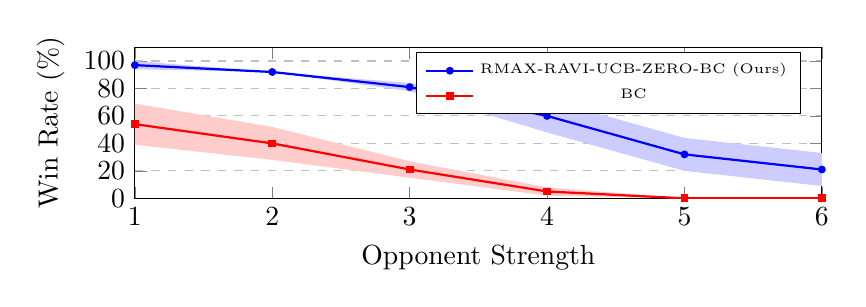
\begin{tikzpicture}
\begin{axis}[
    xlabel={Opponent Strength},
    ylabel={Win Rate ($\%$)},
    xmin=1, xmax=6,
    ymin=0, ymax=110,
    xtick={1,2,3,4,5,6},
    ytick={0, 20, 40, 60, 80, 100},
    legend pos=north east,
    ymajorgrids=true,
    grid style=dashed,
    width=0.85\textwidth,
    height=3.5cm
]

% --- IL as Online Learning ---
% Define the upper bound
\addplot[name path=online_up, draw=none, forget plot] coordinates {
    (1, 100) (2, 92) (3, 84) (4, 72) (5, 44) (6, 33)
};
% Define the lower bound
\addplot[name path=online_down, draw=none, forget plot] coordinates {
    (1, 94) (2, 92) (3, 78) (4, 48) (5, 20) (6, 9)
};
% Fill the region
\addplot[blue!20, forget plot] fill between [of=online_up and online_down];
% Main line
\addplot[color=blue, mark=*, mark size=1pt, thick] coordinates {
    (1, 97) (2, 92) (3, 81) (4, 60) (5, 32) (6, 21)
};
\addlegendentry{\tiny{RMAX-RAVI-UCB-ZERO-BC (Ours)}}


% --- IL as Supervised Learning ---
% Define the upper bound
\addplot[name path=supervised_up, draw=none, forget plot] coordinates {
    (1, 69) (2, 52) (3, 27) (4, 8) (5, 0) (6, 0)
};
% Define the lower bound
\addplot[name path=supervised_down, draw=none, forget plot] coordinates {
    (1, 39) (2, 28) (3, 15) (4, 2) (5, 0) (6, 0)
};
% Fill the region
\addplot[red!20, forget plot] fill between [of=supervised_up and supervised_down];
% Main line
\addplot[color=red, mark=square*, mark size=1pt, thick] coordinates {
    (1, 54) (2, 40) (3, 21) (4, 5) (5, 0) (6, 0)
};
\addlegendentry{\tiny{BC}}

\end{axis}
\end{tikzpicture}
\caption{Win rate of BC vs RMAX-RAVI-UCB-ZERO-BC for different opponent strenghts. \label{fig:winrate_multi}}
\end{figure}

\subsection{Beyond Limitation 2: Imitation Learning from features.}
A second contribution of my thesis has been solving the imitation learning problem when the expert actions are not observed.
This enables the use of massively larger dataset containing onloy the states of the expert or more generally only expert features.
Meaningful features in application could be a frame of a video showing the robot doing a certain task \citep{torabi2018behavioral}.
Formally, we consider a features map $\phi_r: \X\times\A \rightarrow \mathbb{R}^d$ such that $r$ is linear in $\phi_r$ and assume that the expert only reveals a features dataset $\cD_{\phi} = \bc{\phi_r(X^i_E, A^i_E)}^{\tau_E}_{i=1}$,
a dataset which is considerably less informative than $\bc{X^i_E, A^i_E}^{\tau_E}_{i=1}$ when the feature map is infomation-lossy as it happens for example when $\phi_r$ represents a video frame.
Our first fundamental contribution is that, because of the information loss, it is no longer possible to learn 
without access to the enviroment to estimate the transition dynamics.
We make this negative result precise in the following.
\begin{tcolorbox}[
    colback=orange!10!white,
    colframe=orange!80!black,
    %boxrule=0.8pt,
    %arc=2pt,
    %boxsep=2pt,
    %bottom=0pt,
    width=\linewidth
  ]
\begin{theorem} \textbf{Imitation Learning from features requires environment access. \citep{moulin2025optimistically}}
    For any algorithm $\mathrm{Alg}$ having access only to a features dataset, there exists an MDP and an expert policy such that $\mathrm{Alg}$ needs to sample at least $\Omega(\varepsilon^{-2})$   
    state-action sequences and $\Omega(\varepsilon^{-2})$ expert features to learn a $\varepsilon$-optimal policy according to the definition in \eqref{eq:optgoal}.
\end{theorem}
\end{tcolorbox}
Moreover, we match this lower bound in both the number of sample state-action trajectories and in terms of expert features observation, i.e. $\tauE$ with a new algorithm
dubbed FRA-IL \citep{moulin2025optimistically} when the transition dynamics are also linear in same other features map.
The core idea is to reduce imitation learning to a game between a player that plays a sequence of reward functions and a second one playing a sequence of policies.
Finding the right updates for the policy player, solved a problem open in RL theory since 5 years \citep{jin2019provably} which consisted of designing no-regret algorithm for infinite horizon MDPs with linear transitions and rewards.
Key to solve the problem was a new exploration technique combining two classics (UCB \cite{azar2017minimax} and RMAX \citep{brafman2002r}) in a novel way.
The guarantees for FRA-IL read as follows.
\begin{tcolorbox}[
    colback=orange!10!white,
    colframe=orange!80!black,
    %boxrule=0.8pt,
    %arc=2pt,
    %boxsep=2pt,
    %bottom=0pt,
    width=\linewidth
  ]
\begin{theorem} \textbf{Rate optimal upper bounds for Imitation Learning from features.\citep{moulin2025optimistically}}
    For any linear MDP, the algorithm FRA-IL outputs a policy $\piout$ which is $\varepsilon$-optimal sampling $\mathcal{O}(\varepsilon^{-2})$ state-action trajectories and expert features.
\end{theorem}
\end{tcolorbox}
It is important to highlight however that expert interaction as required in the multi agent setting is not needed and the environment rewards are not observed. Only next states are.
Moreover, the bounds can not be improved in terms of $\varepsilon$ because opf our lower bound. Therefore, FRA-IL is rate optimal.

\paragraph{Practical take-away}
From the above theoretical analysis, we learn that exploration in the policy update is crucial. In stark contrast existing algorithm were neglecting this aspect.
We therefore designed, inspired by theory above, a meta algorithm that injects exploration in existing algorithms to learn only from features in simulated robotics.
Remarkably, as shown in \Cref{fig:SOAR}, we noticed a consistent improvement for any base algorithm on which we applied our exploration routine.
\begin{figure}[t]
    \centering
    
    \begin{minipage}[T]{0.7\linewidth}
        \centering
        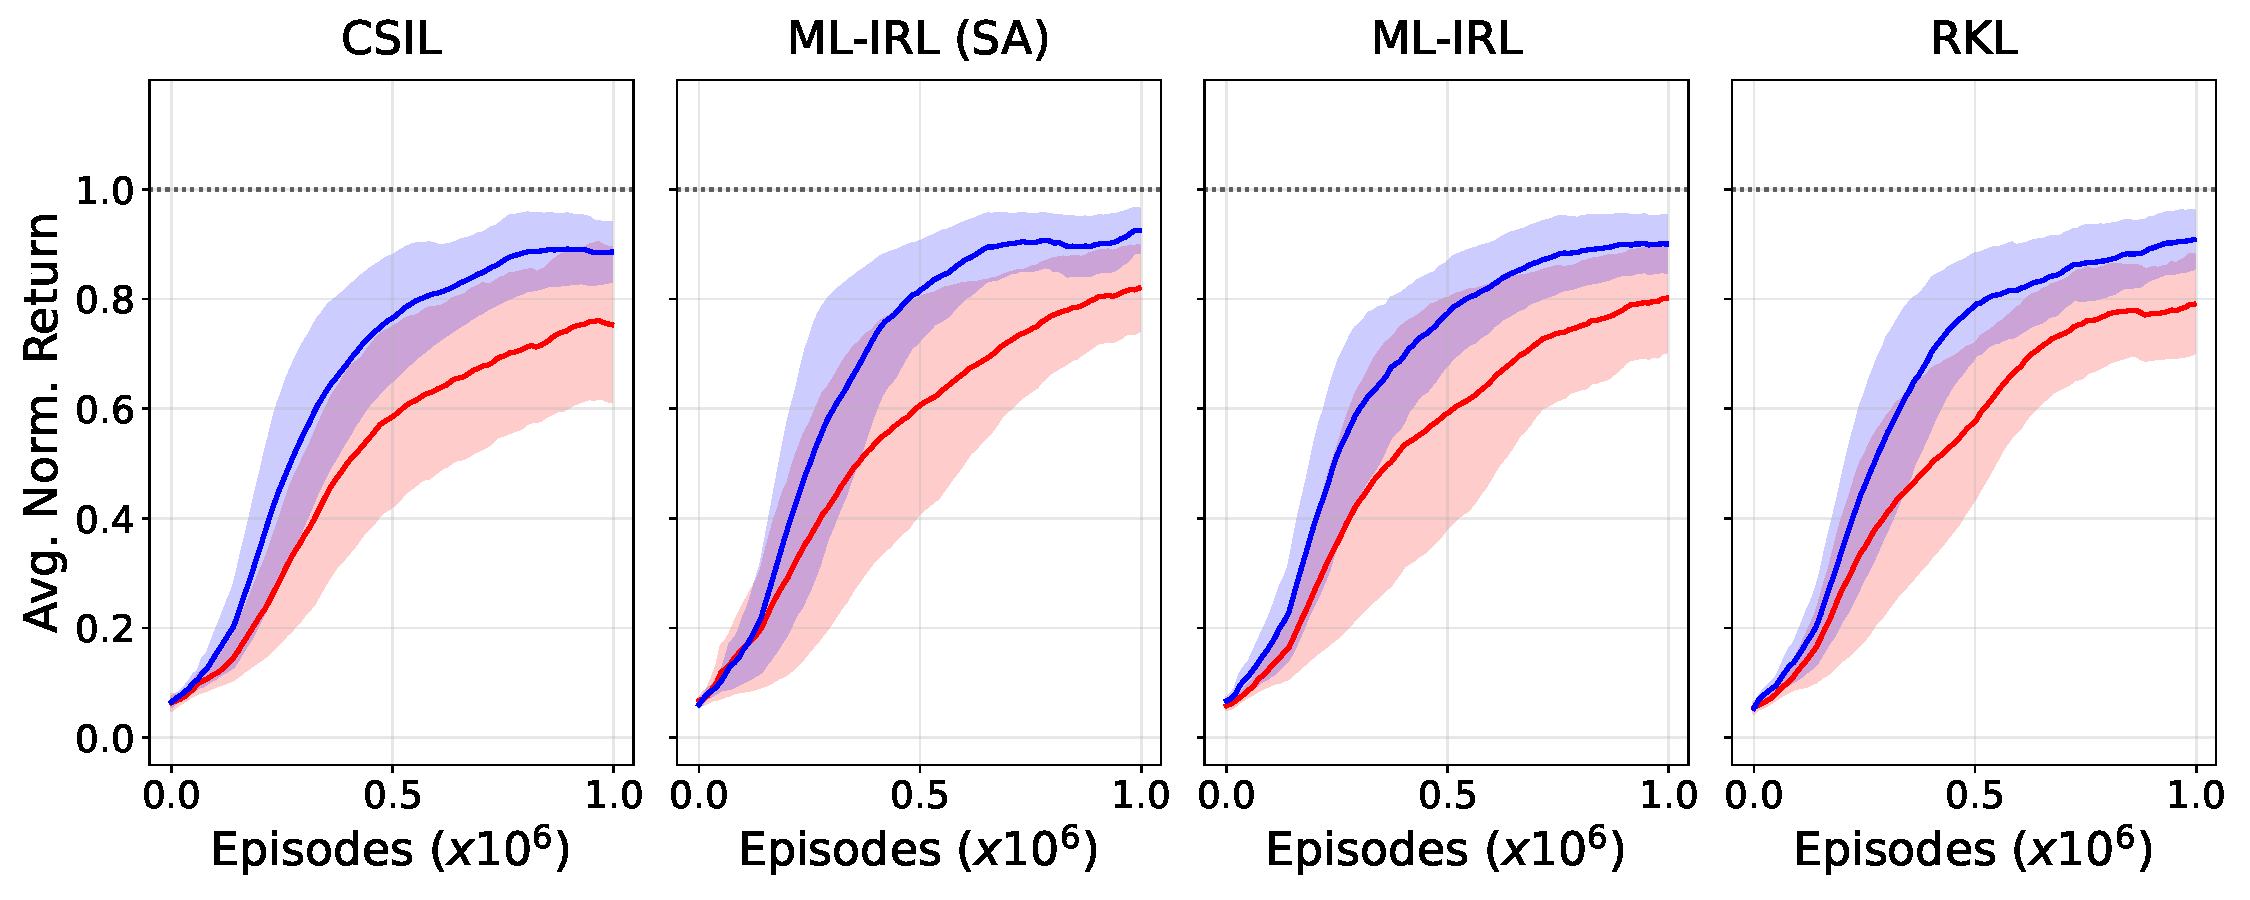
\includegraphics[width=0.8\linewidth]{figures/ch2/method_averages_comparison_with_ci.pdf}
    
        \vspace{3mm}
    
        {\small
        \tikz[baseline=-0.5ex]{\draw[red, thick] (0,0) -- (0.3,0);} Base IL algorithm
        \hspace{0.5cm}
        \tikz[baseline=-0.5ex]{\draw[blue, thick] (0,0) -- (0.3,0);} 
        Base + \textbf{\textcolor{blue}{ensemble-based exploration}}
        }
    \end{minipage}
    \hfill
    \begin{minipage}[T]{0.28\linewidth}
        \centering
        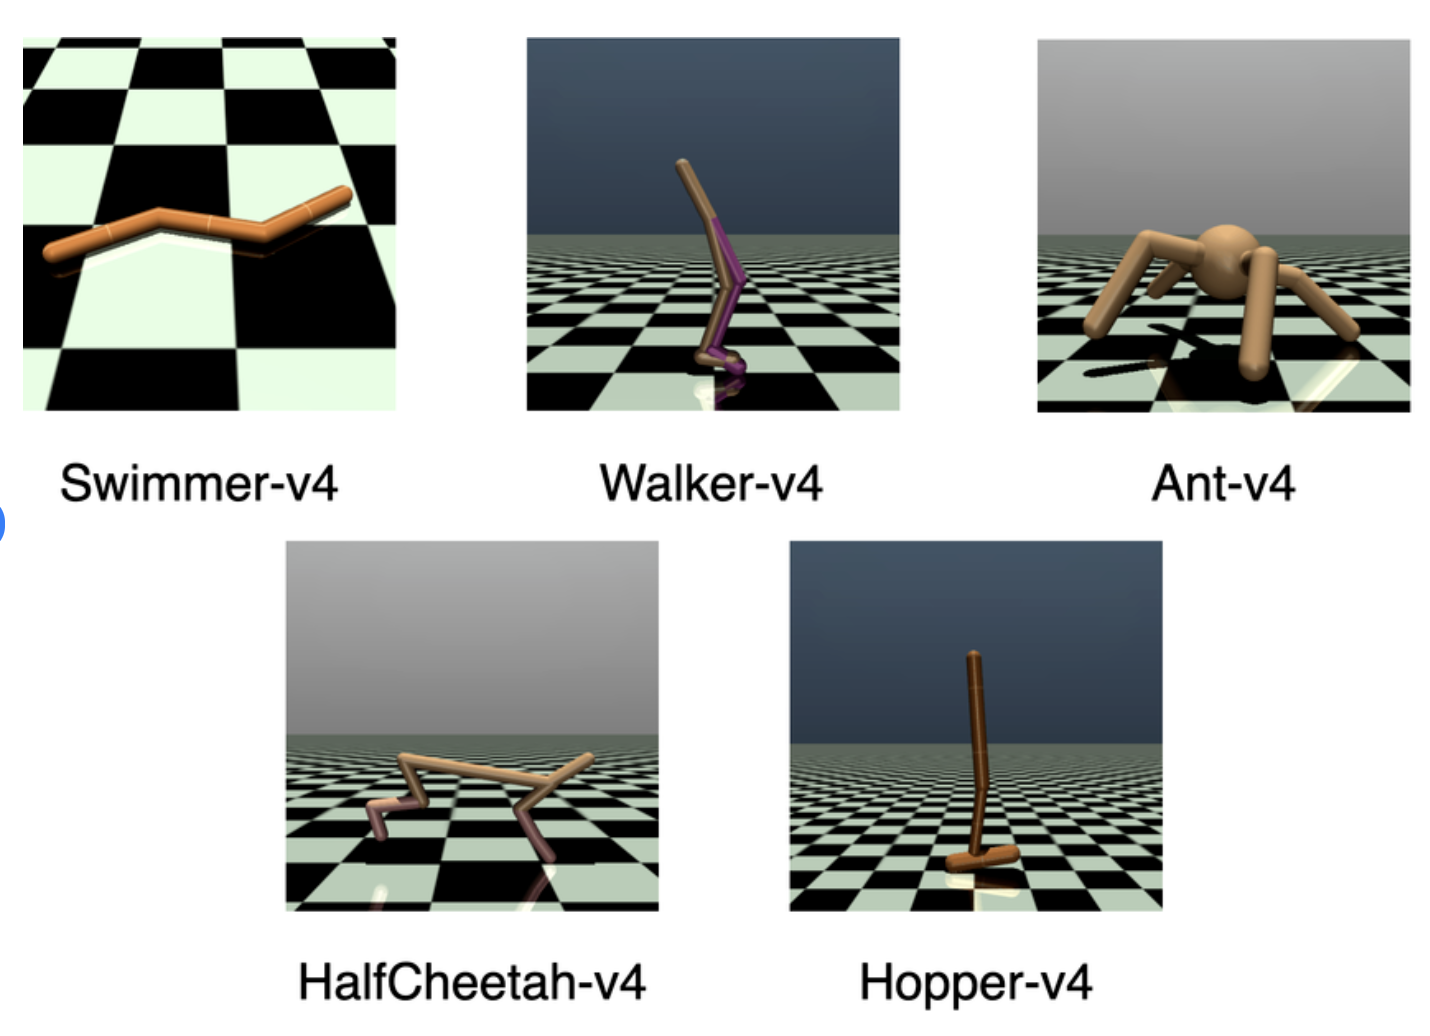
\includegraphics[width=\linewidth]{figures/ch2/mujoco2.png}
    \end{minipage}
    
    \caption{Continuous control imitation learning experiments, results averaged across the 5 environments shown on the right. For any base IL algorithm considered (CSIL \cite{watson2023coherent}, RKL \cite{ni2021f}, ML-IRL \cite{zeng2022structural}) injecting exploration in the policy updates via critics ensembles leads to faster learning.}
    \label{fig:SOAR}
    
    \end{figure}
\section{Beyond Limitation 3: IL without mimicking the expert.}
Folklore imitation learning described above attains the goal in \eqref{eq:optgoal} by 
matching the expert distribution, i.e. mimicking the expert. In other words, the learner
trained via BC tries to choose among the available 
actions with the same probability distribution used by the expert.
However, this is often not possible; especially when the learner is not capable of representing the expert policy. This can often happen in practice.
\begin{example}\textbf{Distillation}
In distillation, a very popular technique in LLMs fine-tuning for mathematical and coding tasks, we train a small model
given some responses generated by a much larger LLM. Given the difference in sizes, the small model can not really represent
the reasoning traces of the larger one. Still, it could generate correct responses via other reasoning steps. However, this can clearly not be obtained 
just maximizing the likelihood of the expert responses. 
\end{example}
\begin{example}\textbf{Learning from a privileged expert.}
In same situation the expert might chooses actions at a given state using external information which is not revealed to the learner, we call this a privileged expert.
For example, in finance, a human investor acts not only looking at the current status of the market but also according to some internal bias
or information aquired elsewhere. Without access to such privileges, the learner can not hope to match 
the expert distribution. However, there is still hope to perform similarly in terms of gained money, even thought by taking different actions.
\end{example}
In our NeurIPS 2025 paper, \citep{moulin2025inverseqlearningrightoffline} we invent the first offline imitation learning which does not mimick the expert.
Formally, the key idea is to avoid assuming access to a class $\PiE$ such that $\expertp \in \PiE$ at the cost of introducing structural assumptions on the environment.
This translates into assumptions on the state action value functions $Q^\pi$ that for a given $\pi:\X\rightarrow \Delta_{\A}$ is defined as $Q^\pi(x,a) = \mathbb{E}^\pi[\sum^{\infty}_{h=0} \gamma^h r(X_h, A_h) | X_0, A_0 = x,a]$.
In particular, we consider access to a class $\cQ$ such that it is expressive enough to either:
(\textbf{Case I}) represent the state-action value functions of any generated policy by the algorithm we run, or 
(\textbf{Case II}) the expert state-action value function $Q^{\expertp}$ is representable by the class $\cQ$.
In practice, one should think of the class $\cQ$ of the functions that can be represented by a fixed neural network architectures by changing the weights.
Our first, result is to show that (\textbf{Case II}) is more difficult than (\textbf{Case I}).
\begin{tcolorbox}[
    colback=orange!10!white,
    colframe=orange!80!black,
    %boxrule=0.8pt,
    %arc=2pt,
    %boxsep=2pt,
    %bottom=0pt,
    width=\linewidth
  ]
\begin{theorem} \textbf{Under Case II offline learning is not possible.}
There exists a family of MDPs and expert pairs such that if $\cQ$ satisfies \textbf{Case I},
then the algorithm SPOIL \citep{moulin2025inverseqlearningrightoffline} learns a $\varepsilon$-optimal policy observing $\cO(\varepsilon^{-2})$ offline expert data, without any dependence on $\abs{\PiE}$.    
At the same time, if $\cQ$ only satisfies \textbf{Case II}, no algorithm can learn.
\end{theorem}
\end{tcolorbox}
The above thereom gives a positive result under \textbf{Case I}, but how to learn under the weaker assumption (\textbf{Case II}) ?
The answer resides into expert interactions. We design an algorithm, named OVI, such that 
queries the expert along the learner trajectory to learn an $\varepsilon$-optimal policy in \textbf{Case II} without any dependence
on the expert complexity but only on the class $\cQ$. 
The idea to design the algorithm is to circumvent the likelihood maximization performed by BC but working directly with the objective in \eqref{eq:optgoal}. Following this philosophy, 
we cast a game between a policy player and this time a $Q$-values player, not a reward player as done in the above section.
\begin{tcolorbox}[
    colback=orange!10!white,
    colframe=orange!80!black,
    %boxrule=0.8pt,
    %arc=2pt,
    %boxsep=2pt,
    %bottom=0pt,
    width=\linewidth
  ]
\begin{theorem} \textbf{Expert interaction enables efficient learning under Case II.}
Given $\cQ$ satisfying \textbf{Case II}, OVI learns a $\varepsilon$-optimal policy after $\cO(\varepsilon^{-4})$ expert 
queries or $\cO(\varepsilon^{-2})$ if $\cQ$ is convex.
\end{theorem}
\end{tcolorbox}
\paragraph{Practical take-away}
The above theoretical findings give us important practical take away for the distillation setting, where the expert policy 
is parameterized by way more parameters than the learner one. In these settings, maximizing the 
likelihood of the expert actions as BC or DAgger \citep{Ross:2011} do, is not a good idea because the small network
is not capable of matching exactly the probability used by the expert policy. 
In contrast our method, OVI, focus on obtaining the same performance, even if this is achieved via different actions.
Our experiments in control environments, see \Cref{fig:size_scaling}, confirm that as the networks size gap between the expert and the learner increases our method OVI 
becomes stronger and stronger compared to the maximum likelihood based approachs (BC and DAgger).

\begin{figure*}[!t]
    \centering
    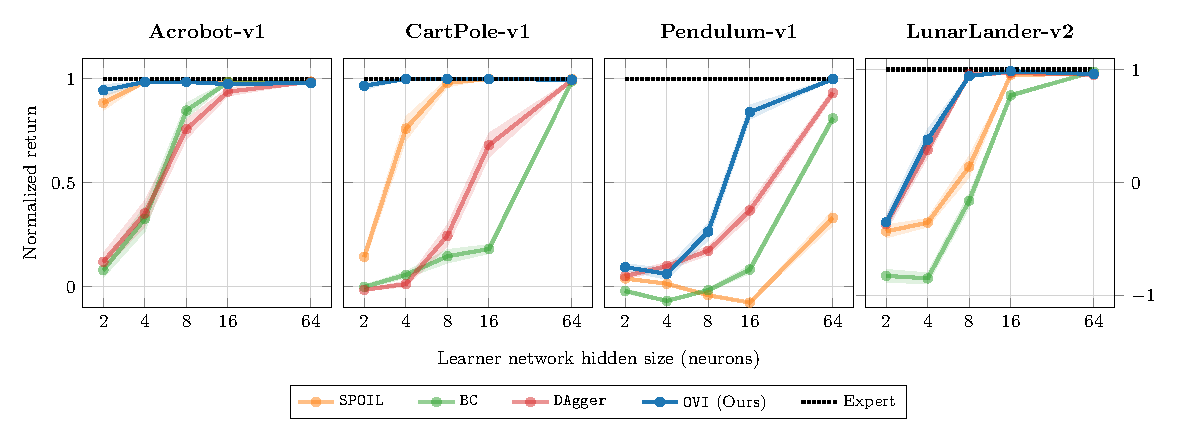
\includegraphics[width=\linewidth]{figures/size_scaling_figure_pendulum.pdf}
    \caption{
    \textbf{OVI enables smaller learner networks.} Average return ($y$-axis) as a function of the learner network hidden size ($x$-axis), over $50$ seeds and $10$ expert trajectories. We compare with offline and interactive policy-based methods (BC, DAgger) , and the offline value-based method SPOIL. Expert network is of size $64$, thus expert policy realizability holds only at the rightmost point of the $x$-axis. OVI outperforms all baselines across all network sizes. \label{fig:size_scaling}}
    \vspace{-0.8em}
\end{figure*}
\section{Beyond Limitation 4: robust offline alignment.}
The last part of my thesis focuses on learning from preferences that can be seen as an extension of imitation learning 
where the learner is informed not only about what to imitate but also about which actions to avoid. 
Among existing approaches for learning from preferences (a.k.a. alignment), \emph{Direct Preference Optimization} (DPO) \citep{rafailov2023direct} has gained widespread adoption due to its strong empirical performance and simplicity of implementation: indeed, DPO elegantly bypasses the intermediate step of learning a reward function from the preference dataset. 
\begin{figure*}[t]
    \centering
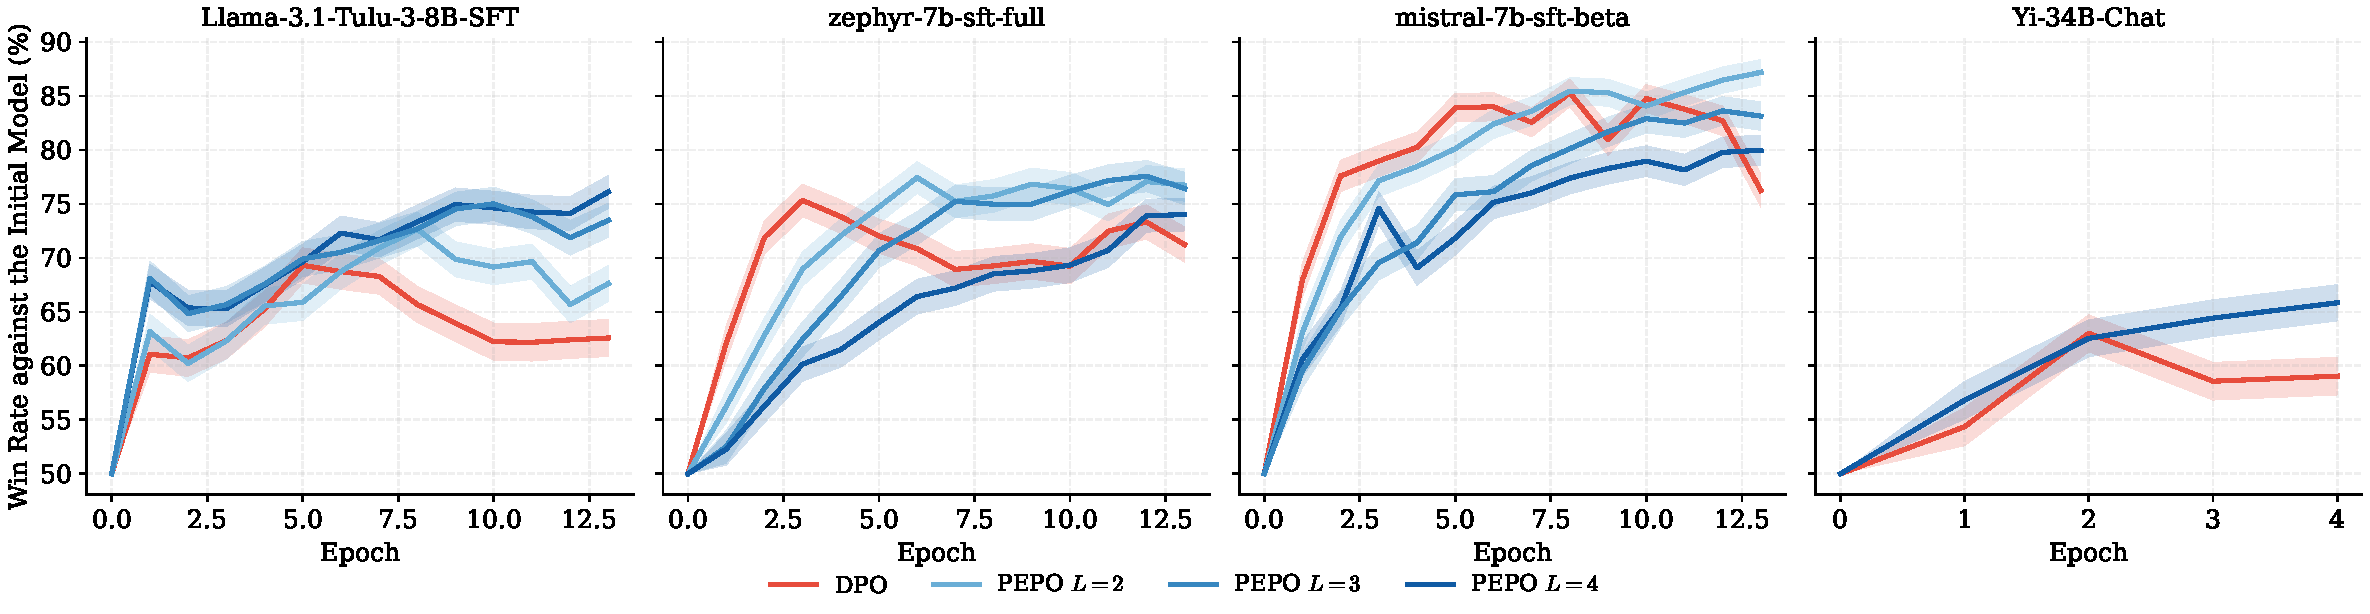
\includegraphics[width=\textwidth]{figures/ch5/win_rate_initial.pdf}
    \caption{Win rate (\%) against the initial model on AlpacaEval2 across training epochs. Shaded regions indicate standard error of the mean across per-instruction preferences. We compare DPO and PEPO with varying ensemble sizes $L$. %As expected by our theory, PEPO does not show signs of overoptimizationconsistently outperforms DPO., %with more pronounced improvements on models with stronger initial GPT-4 win rates (\texttt{Yi-34B-Chat} (27.5\%) and \texttt{Llama-3.1-Tulu-3-8B-SFT} (8.6\%) show larger gains compared to \texttt{Mistral-7B} (4.1\%) and \texttt{Zephyr-7B} (3.5\%)).
    }
    \label{fig:winrate-initial}
\end{figure*}
%However, on the negative side, DPO is known to suffer from the over-optimization issue: the algorithm can quickly overfit on the preference dataset leading to models which are worse than the starting one \citep{park2024disentangling,gao2023scaling,xu2024dpo}. 
Despite these advantages, DPO is known to suffer from \emph{over-optimization}: as training progresses, improvements in optimizing the training loss do not necessarily translate into better generation quality, and may even degrade performance relative to the initial model \citep{gao2023scaling, park2024disentangling, xu2024is}.
Moreover, early stopping using the validation loss as a criterion is not reliable because it is only a loose proxy for what really matters, i.e. the quality of the responses that the model can generate in practice. 
Several new DPO variants 
%have been proposed to 
mitigate over-optimization via \emph{pessimistic regularization}. 

Notably, approaches such as $\chi^2$-regularized preference optimization ($\chi^2$PO) \citep{huang2024correcting} and DPO augmented with supervised fine-tuning (DPO+SFT) \citep{liu2024provably} achieve guarantees that depend only on a \emph{single-policy} concentrability coefficient $C^\star = \sum_{x,a\in \X\times\A} \initial(x) \frac{(\pi^\star(a|x))^2}{\pidata(a|x)}$, which is the theoretical certificate of robustness to over-optimization \citep{huang2024correcting}. 
In contrast, DPO is guaranteed to find a good approximation of the maximizer of \eqref{eq:PEPOgoal} only when $C^{\mathrm{all}} = \sup_{\pi:\X\rightarrow \Delta_{\A}}\sum_{x,a\in \X\times\A} \initial(x) \frac{(\pi^\star(a|x))^2}{\pidata(a|x)}$ is bounded.

However, they rely on the assumption that we have access to the data-generating distribution $\pidata$, an assumption 
which is often broken in practice, for instance, when smaller models are post-trained 
using preference data (e.g.  the UltraFeedback dataset  \citep{cui2023ultrafeedback} ) generated by larger, proprietary systems 
whose logits can not be accessed when fine-tuning the smaller models. 
In the last chapter of my thesis, I remove this limitation with a new algorithm: PEPO.
The central idea behind PEPO is to resort to \emph{pessimism via ensembles}: a technique as simple as unexplored in the context of LLM alignment, especially in the DPO setting.
Concretely, PEPO trains an ensemble of $L$ lightweight DPO-style policies on disjoint subsets of the preference dataset, implemented via low-rank adapters \citep{hu2022lora}. Finally, at generation time, we use a certain notion of ensemble agreement to generate responses either via rejection sampling or approximating the (otherwise intractable) response-level normalization constant to the token-level counterpart.
All in all, we obtain the following formal guarantees.
\begin{tcolorbox}[
    colback=orange!10!white,
    colframe=orange!80!black,
    %boxrule=0.8pt,
    %arc=2pt,
    %boxsep=2pt,
    %bottom=0pt,
    width=\linewidth
  ]
\begin{theorem} \textbf{PEPO avoids over-optimization without knowing $\pidata$.}
PEPO learns, with probability $1-\delta$, a $\varepsilon$-optimal policy for \eqref{eq:PEPOgoal}, when given a dataset of size $\cO\br{\nicefrac{C^\star \log(1/\delta)}{\varepsilon^2}}$ preferences.
\end{theorem}
\end{tcolorbox}
Notably, in the above theorem there is no dependence at all on $C^{\mathrm{all}}$ and the dependence on $C^\star$ is better then what obtained in prior works. 
Finally, the result is attained without knowing $\pidata$.
Practically, we tested our method in which $\pidata$ is unknown because the responses 
in the dataset are generated by
a non-public model and noticed that while the performance of DPO increases initially,
 it decreases drastically after a certain number of epochs (see \Cref{fig:winrate-initial}). In contrast, PEPO's performance increases in a monotonic manner 
 in all four cases which differ in the choice of the initial model $\piref$.
The performance in this context is measured with the LLM-as-a-judge protocol.
A large LLM (Llama-70B) has to decide the winner among one response generated by the starting model $\piref$
and one from the model fine tuned via DPO or PEPO. Then, the performance is the percentage of wins that the fine-tuned model attains.

It can also be notice that the ensemble size $L$ has a strong effect on the performance. Our theory provides 
guidance for the optimal choice. In particular, if $L$ is too small than we can not guarantee
that we estimate pessimistically the true reward gap.
On the contrary, when $L$ is too large, then each LoRA model is trained with a too small amount of data. All in all, the best choice of $L$ is the 
smallest one among the values small enough to guarantee pessimism. This change depending on the initial model $\piref$. 
For example, it can be seen in \Cref{fig:winrate-initial} that for Llama, with $L=2$ we still suffer overoptimization, i.e. the performance drops after some epochs.
In contrast, $L=2$ is the best choice for Zephyr.
Finally, we remark that PEPO remains effective at scale as confirmed by our finetuning 
experiment on a 34B model, Yi-34B.

\section{Conclusions}

\newpage
\bibliographystyle{plainnat}
\bibliography{references}
\newpage
\appendix

\end{document}
